\documentclass[a4paper]{book}


\usepackage[student]{Lecture}
%\lhead{Cours n°1 : Lithium au sein du tableau périodique}
\lhead{\leftmark} \chead{} \rhead{4.13}
\lfoot{IUT d'Orsay - BUT 2 MAT - 2025-2026} \cfoot{
\includegraphics[height=0.5cm]{cc-by-nc-sa.png}}  \rfoot{Jean-François Olivieri \quad \thepage}

\begin{document}

\begin{comment}
\begin{titlepage}
  \begin{sffamily}
  \begin{center}

    % Upper part of the page. The '~' is needed because \\
    % only works if a paragraph has started.
    \includegraphics[height=4cm]{logo.png}~\\[0.5cm]

    \textsc{\LARGE Université Paris-Saclay}\\[0.5cm]
    
    \textsc{\Large IUT d'Orsay - Département de Chimie}\\[0.5cm]
    
    \textsc{\large BUT 2, module 3.06 - Propriété des matériaux}\\[3.0cm]

    % Title
    \HRule \\[0.4cm]
    { \huge \bfseries Matériaux pour l'énergie\\[0.4cm] }

    \HRule \\[0.4cm]
    
       
    \textsc{\Large  Une introduction aux batteries}\\[0.5cm] 
    
    \textsc{\Large  Année 2023-2024}\\[5.0cm]
    


    % Author and supervisor
    \begin{minipage}{0.48\textwidth}
      \begin{flushleft} \large
        \faPencil ~ Jean-François Olivieri\\
        ~ \faPaperPlane ~ jean-francois.olivieri@universite-paris-saclay.fr
      \end{flushleft}
    \end{minipage} \hfill
    \begin{minipage}{0.48\textwidth}
      \begin{flushleft} \large
      	\faUsers ~ Lionel Tinat \\
      	~ \faPaperPlane ~ lionel.tinat@universite-paris-saclay.fr
        \faUsers ~ Frederic Banse \\
        ~ \faPaperPlane ~ frederic.banse@universite-paris-saclay.fr
      \end{flushleft}
    \end{minipage}

    \vspace{2.8cm}

   	{\scriptsize Photo de garde tirée de \href{https://chemistry-europe.onlinelibrary.wiley.com/toc/25666223/2023/6/2}{Batteries \& Supercaps, Improving Electrochemical Activity of P2-type \ce{Na_{2/3}Mn_{2/3} Ni_{1/3}O2} by Controlling its Crystallinity}, R. Kataoka \& co-workers.}

    % Bottom of the page
    
    {\scriptsize \doclicenseThis}

  \end{center}
  \end{sffamily}
\end{titlepage}
\end{comment}

\tableofcontents

\setcounter{chapter}{1}
\chapter{Potentiel chimique et construction d'un diagramme de phase}

L'utilisation du potentiel chimique dans le cadre des mélanges permet de faire le lien entre les interactions des constituants chimiques et la forme des diagrammes de phase. Ce lien est extrêmement important pour faire le lien entre modèle et expérience, structure et propriété.

De plus, nous observerons que des modèles assez élémentaire permette de rendre compte qualitativement ou quantitativement des phénomènes thermiques des mélanges : coexistence de phase solide et liquide, démixtion des solides en un mélange hétérogène$\ldots$

\section{Expression du potentiel chimique}
\subsection{Potentiel chimique d'un mélange de gaz parfait}

\begin{center}
\begin{minipage}{0.5\textwidth}

\includegraphics[width=\textwidth]{figures/Fig07}
\captionof{figure}{Mélange de deux gaz parfaits formant un système fermé $n = n_A + n_B$}
\end{minipage}
\end{center}

Le potentiel chimique d'un gaz parfait est déductible de la $3^e$ identité thermodynamique et de la loi de Dalton : 
\begin{align*}
\begin{cases}
\left(\frac{\partial \mu_A}{\partial P} \right)_{T, x_A, x_B} &= V_{m, A} \\
P V_{m,A} &= RT \\
P_A &= x_A P
\end{cases} &\implies \left(\frac{\partial \mu_A}{\partial P_A} \right)_{T, x_A, x_B} = V_{m, A} \\ &\implies \mu_A (T, P, x_A) = \mu_A^\circ (T) + RT \ln  \frac{P}{P^\circ} + RT \ln x_A \\
&\implies \mu_A (T, P, x_A) =  \mu^\star_A (T, P) + RT \ln x_A
\end{align*}

L'enthalpie de mélange s'écrit donc sous la forme :
\begin{align*}
\Delta G_m &= \underbrace{n_A \mu_A (T, P, x_A) + n_B \mu_B (T, P, x_B)}_{\text{mélange}} -  \underbrace{\left( n_A \mu^\star_A (T, P) + n_B \mu^\star_B (T, P) \right)}_{\text{corps purs}} \\
&= n RT \left( (1-x_B) \ln (1- x_B) + x_B \ln ( x_B )\right)
\end{align*}

\definition{
Puisque un gaz parfait est par définition constitué de particules ponctuelles et sans interactions, l'enthalpie de mélange est nécessairement nulle. La force motrice du mélange de gaz parfait est purement statistique (et par conséquent, entropique).

Tout système qui n'est pas un gaz, et qui présente ces propriétés, est dit idéal.
}


\subsection{Potentiel chimique dans un mélange quelconque}

\definition{
Le potentiel chimique d'un constituant chimique $i$ s'écrit sous la forme : 
\begin{align*}
\mu_i (T, P, \text{composition}) = \mu_i^{ref} (T, P) + RT \ln \left( a_i (T, P, \text{composition} ) \right) 
\end{align*}
où $\mu_i^{ref}$ est le potentiel chimique de référence et $a_i$ l'activité du constituant $i$.}

Le potentiel chimique de référence dépend :
\begin{itemize}
\item du choix de la coordonnée décrivant la composition du mélange, comme par exemple la fraction molaire, la concentration, la molalité, $\ldots$
\item du choix de l'état de référence du constituant $i$.
\end{itemize}

Par conséquent, le terme de mélange mesure un écart à cet état de référence.


\subsection{États de référence}

Dans un mélange, on considère souvent deux états limites de référence : 
\begin{itemize}
\item un des constituant est majoritaire (solvant), on se sert dans ce cas de l'état corps pur,
\item un des constituant est minoritaire (soluté), on se sert dans ce cas de l'état infiniment dilué.
\end{itemize}

\subsubsection{Etat de référence corps pur (ERCP)}

\definition{
Dans le cas où on prend l'état de référence corps pur pour un constituant chimique $i$ d'un mélange, on a :
\begin{align*}
\mu_i (T, P, x_i) = \mu_i^{\star} (T, P) + RT \ln \left( a_i^\star (T, P, x_i) \right)
\end{align*}
}

Dans l'état de référence corps pur, on pose que l'activité chimique s'écrit comme : 
\begin{align*}
a_i^\star (T, P, x_i) = \gamma_i^\star (T, P, x_i) \cdot x_i
\end{align*}

avec $\gamma_i^\star$ est le c{\oe}fficient d'activité du constituant $i$ dans l'ERCP.

Dans la limite du corps pur, on doit retrouver une activité de $1$ :
\begin{align*}
\lim_{x_i \to 1} \gamma_i^\star (T, P, x_i) = 1
\end{align*}

Si le constituant $i$ est largement majoritaire, alors $x_i \to 1$, on retrouve donc une activité de $1$.

\begin{center}
\begin{minipage}{0.48\textwidth}

\includegraphics[width=\textwidth]{figures/Fig01a}
\end{minipage}\hfill\begin{minipage}{0.48\textwidth}
\captionof{figure}{Représentation schématique de l'évolution du potentiel chimique lorsque l'on s'éloigne du corps pur}
\label{fig:01a}
\end{minipage}
\end{center}

Le coefficient d'activité est une mesure relative de la stabilisation du solvant par les interactions soluté-solvant. Comme représenté à la Fig. \ref{fig:01a}, si : 
\begin{align*}
\gamma_i^\star > 1 &\implies \text{les interactions solvant-soluté déstabilisent le solvant} \\
\gamma_i^\star < 1 &\implies \text{les interactions solvant-soluté stabilisent le solvant} \\
\end{align*}
Cet écart à l'idéalité est appelé terme d'excès.

\subsubsection{Etat de référence infiniment dilué (ERID)}

\definition{
Dans le cas où on prend l'état de référence infiniment dilué pour un constituant chimique $i$ d'un mélange, on a :
\begin{align*}
\mu_i (T, P, x_i) = \mu_i^{\infty} (T, P) + RT \ln \left( a_i^\infty (T, P, x_i) \right)
\end{align*}
}

Dans l'état de référence corps pur, on pose que l'activité chimique s'écrit comme : 
\begin{align*}
a_i^\infty (T, P, x_i) = \gamma_i^\infty (T, P, x_i) \cdot x_i
\end{align*}

avec $\gamma_i^\star$ est le c{\oe}fficient d'activité du constituant $i$ dans l'ERCP.

Dans la limite d'une solution infiniment diluée, on doit retrouver une activité proportionnelle à la fraction molaire :
\begin{align*}
\lim_{x_i \to 0} \gamma_i^\infty (T, P, x_i) = 1
\end{align*}

Si le constituant $i$ est largement majoritaire, alors $a^\infty_i \to x_i$, on retrouve donc une activité proportionnelle à la quantité de matière.

\subsubsection{Interprétation}

Considérons un système thermodynamique contenant deux constituants \ce{A} et \ce{B}.

\begin{figure}[H]
\begin{center}
\begin{minipage}{0.6\textwidth}
\subfloat[\label{fig:Chp4-01b}]{
\includegraphics[height=4.0cm]{figures/Fig01b}}
\hspace{0.5cm}\subfloat[\label{fig:Chp4-01c}]{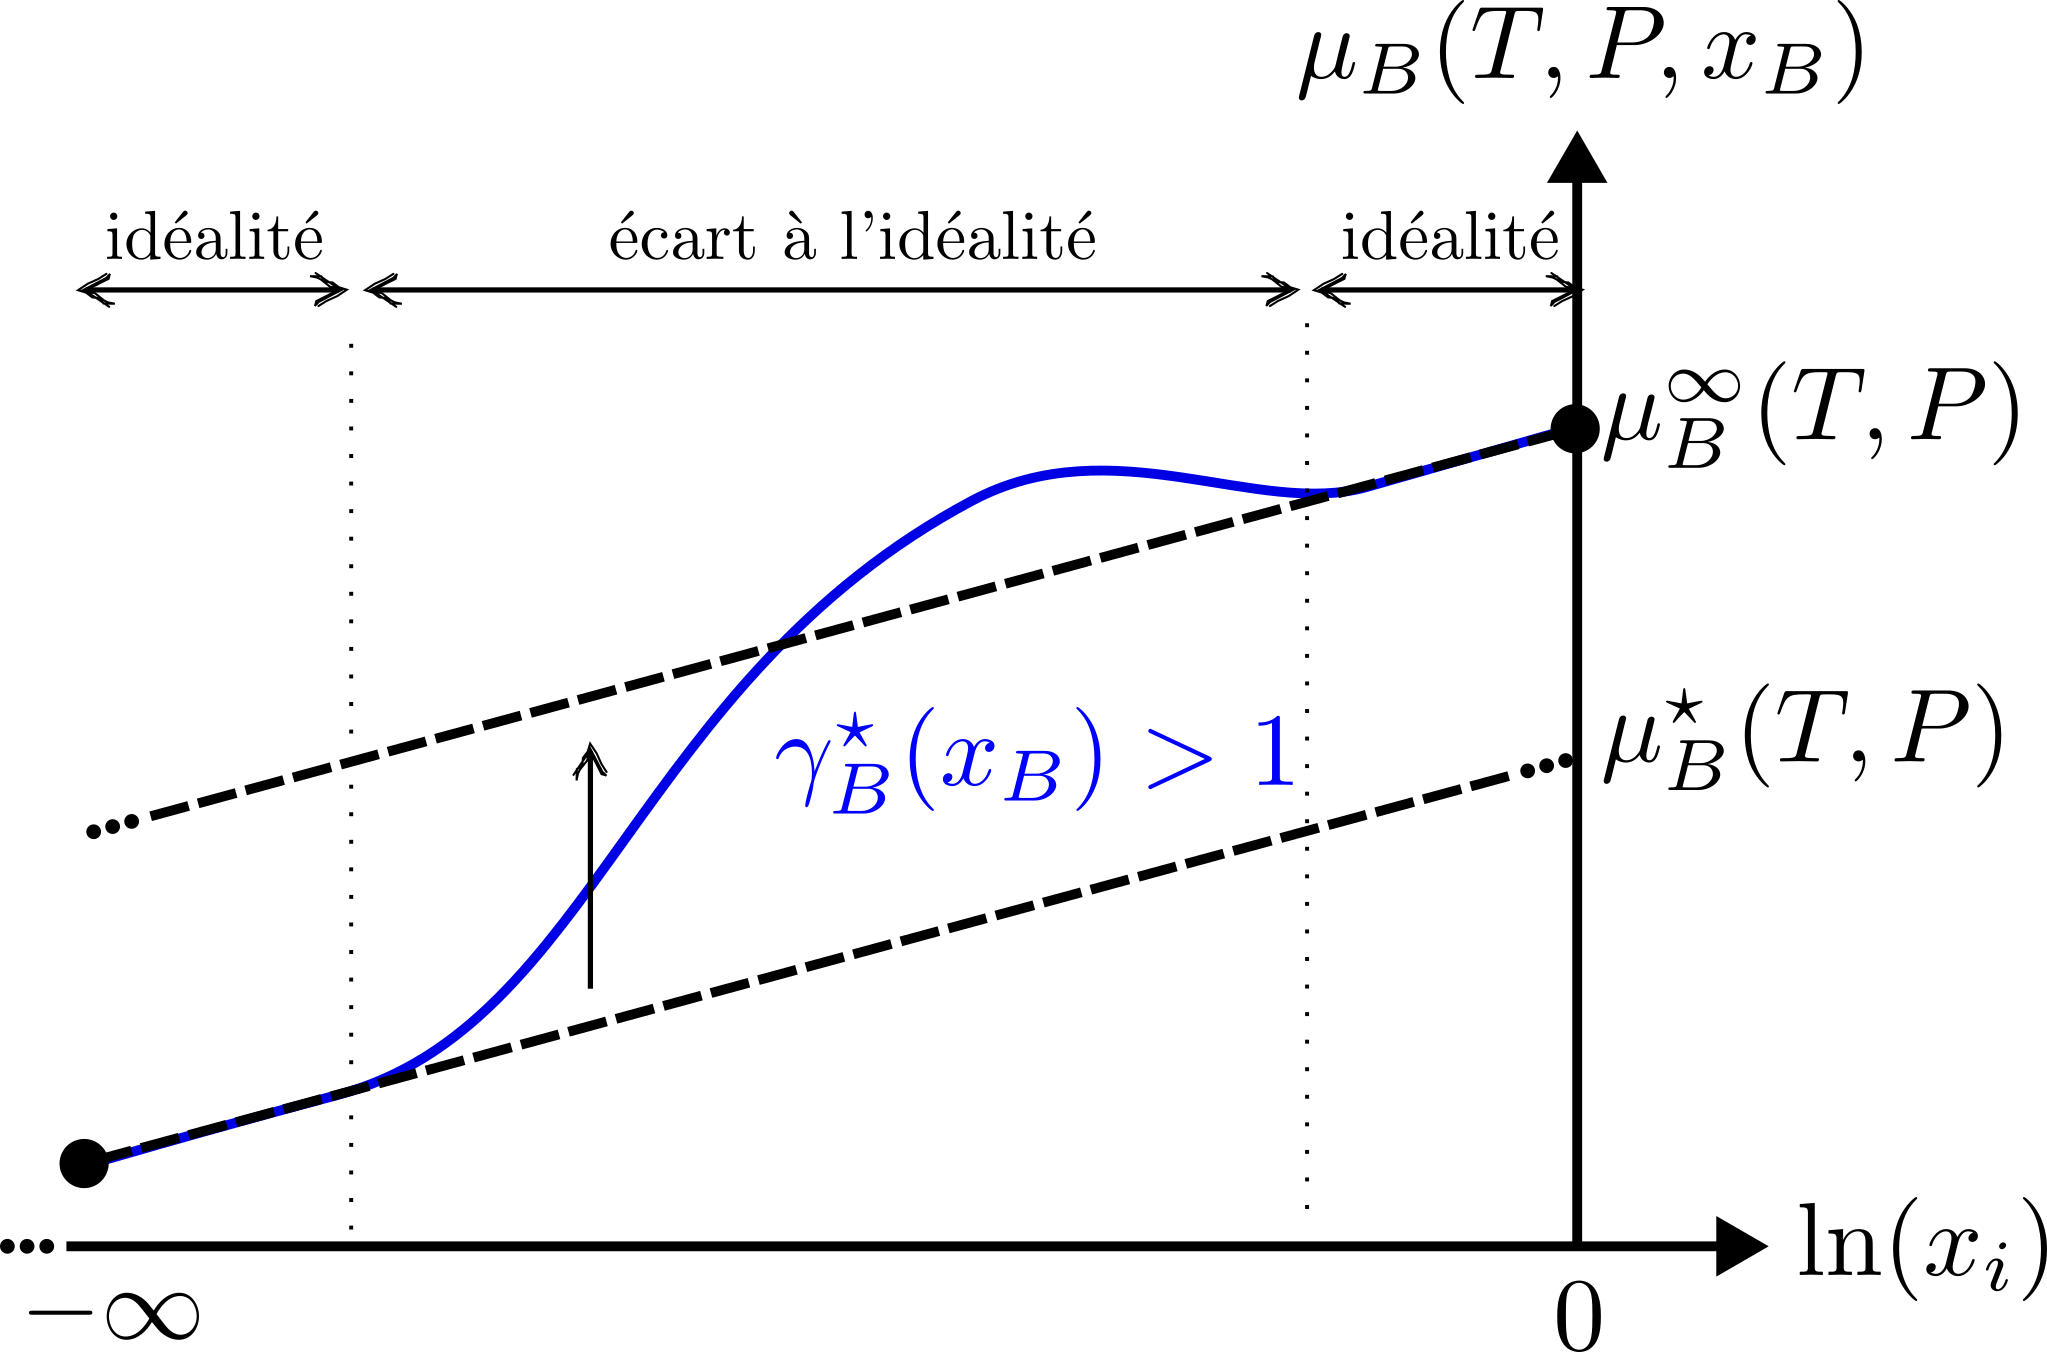
\includegraphics[height=4.0cm]{figures/Fig01c}}
\caption{Evolution du potentiel chimique d'un constituant B en fonction de la fraction molaire en échelle logarithmique dans le cas d'une interaction \ce{A-B} plus \ref{fig:Chp4-01b} favorable (\ref{fig:Chp4-01c} défavorable) que les interactions \ce{A-A} et \ce{B-B}}
\label{fig:04-01}
\end{minipage}
\end{center}
\end{figure}

\`{A} la Fig. \ref{fig:Chp4-01b}, on observe que le potentiel chimique de \ce{B} diminue lorsque les interactions \ce{A-B} sont plus favorables que les interactions \ce{A-A} et \ce{B-B}. Dans un tel système, le coefficient d'activité dans l'ERCP (resp. l'ERID) sont plus petit (resp. grand) que 1.

\`{A} la Fig. \ref{fig:Chp4-01c}, on observe le contraire.


Dans un système parfaitement idéal, le coefficient d'activité vaut $1$ à tout composition
\begin{align*}
\forall x_i, \gamma_i^\star (x_i) = \gamma_i^\infty (x_i) = 1
\end{align*}


Une des conséquences immédiate est que : 
\begin{align*}
\mu_i^{\star} (T, P) = \mu_i^{\infty} (T, P) 
\end{align*}

\section{Miscibilité totale, partielle ou nulle}

Lorsque l'on mélange deux constituants \ce{A} et \ce{B}, il est possible d'observer l'un des trois types de comportements suivants :
\begin{enumerate}
\item les deux constituants sont totalement miscibles dans une phase homogène :
\begin{align*}
\ce{(1-x) A(s) + x B(s) -> A_{1-x} B_x (s)}
\end{align*}
\item les deux constituants sont partiellement miscibles :
\begin{align*}
A_{1-x} B_x(s) \to (1-x^\beta) A_{1-x_B^\alpha}B_{x_B^\alpha} (\alpha) + x^\beta A_{1-x_B^\beta}B_{x_B^\beta} ( \beta )
\end{align*}

avec $x^\beta$ (resp. $x^\alpha$) la fraction molaire de phase $\beta$ (resp. $\alpha$) et $x_B^ \beta$ (resp. $x_B^\alpha$) la fraction molaire (limite de solubilité) de \ce{B} dans la phase $\beta$ (resp. $\alpha$)
\item les deux constituants sont non miscibles, auquel cas, pour une fraction $x$ (resp. $1 - x$) de \ce{B} (resp. \ce{A}), on forme un mélange hétérogène constitué d'une phase représentant $x$ \si{\percent} (resp. $1 - x$ \si{\percent}) de phase \ce{B} (resp. \ce{A}) pure.
\end{enumerate}

Dans tout ce qui suit, on va chercher à comparer la stabilité des différents types de mélange en les comparant aux corps purs en utilisant l'enthalpie libre de mélange, définie comme : 
\begin{align*}
\Delta G_m = G_{\text{mélange}} - G_{\text{corps purs}}
\end{align*}

Le processus chimique de mélange est bien entendu bien plus complexe (chauffe, refroidissement, cristallisation, $\ldots$). Cependant, l'enthalpie libre de mélange permet d'établir une comparaison entre l'état initial (corps purs) et l'état final (mélange) et ainsi de comparer la stabilité.


\subsection{Théorie des mélanges}

\begin{align*}
\ce{(1-x) A(s) + x B(s) -> A_{1-x} B_x (s)}
\end{align*}

L'enthalpie d'un tel système s'écrit sous la forme : 
\begin{align*}
G_s (T, P, n_A, n_B) = n_A \mu_A(T, P, x) + n_B \mu_B (T, P, x)
\end{align*}

\subsection{Idéalité}
Dans le cas où les interactions \ce{A-A} et \ce{B-B} sont équivalentes aux interactions \ce{A-B}, les c{\oe}fficients d'activités valent $1$ à toute composition. On parle d'idéalité du mélange.

\definition{
Dans un mélange idéal, le mélange est décrit par les égalités suivantes : 
\begin{align*}
\Delta H_m &= 0 \\ 
\Delta S_m &= - n^s R \left[ (1-x) \ln (1-x) + x \ln (x) \right] \quad \text{ avec } n^s = n_A + n_B
\end{align*}
Par conséquent, l'enthalpie libre d'un mélange s'écrit comme : 
\begin{align*}
\Delta G_m = n^s R T \left[ (1-x) \ln (1-x) + x \ln (x) \right]
\end{align*}
}

L'enthalpie de mélange nulle traduit le fait que $H_{AB} = H_{A} + H_{B}$, soit que toutes les interactions dans le mélange \ce{AB} sont de même force que les interactions dans les corps purs \ce{A} et \ce{B} réunis. L'enthalpie libre de mélange est donc purement entropique et négative à toute composition, ce qui traduit la stabilité du mélange idéal par rapport aux corps purs.

\begin{center}
\begin{minipage}{0.58\textwidth}

\includegraphics[width=\textwidth]{figures/Fig04a}
\end{minipage}\hfill\begin{minipage}{0.38\textwidth}
\captionof{figure}{Evolution de l'enthalpie libre de mélange dans le cas d'une solution solide idéale}
\end{minipage}
\end{center}

\subsection{Solution régulière}
\definition{Une solution régulière est un modèle de mélange où l'enthalpie de mélange peut s'écrire sous la forme :
\begin{align*}
\Delta H_m = n^s J_{AB} x_A \cdot x_B
\end{align*}

Le terme $J_{AB}$, en \si{\joule\per\mole}, est un paramètre mesurant les interactions entre les constituants \ce{A} et \ce{B} du mélange, supposé indépendant de la température et de la composition. 

Afin de comparer $J_{AB}$ à l'énergie cinétique moléculaire, on utilise souvent $\chi_m$, son expressioin adimentionnée : 
\begin{align*}
\Delta H_m = n^s \underbrace{RT \chi_m}_{J_{AB}} x_A \cdot x_B
\end{align*}
Attention, cela ne signifie pas que l'on considère que $J_{AB}$ est proportionnel à la température !
}

Dans ce modèle, l'enthalpie de mélange s'exprime comme : 
\begin{align*}
\Delta G_m = \underbrace{n^s RT \left[ (1-x) \ln (1-x) + x \ln (x) \right]}_{idéal} +  \underbrace{n^s J_{AB} x (1-x)}_{excès}
\end{align*}

Or, comme $G = G_A^\star + G_B^\star + \Delta G_m$, on peut facilement remonter à l'expression du potentiel chimique, puisque :

\begin{align*}
  \mu_A (T, P, x) &= \left( \frac{\partial G}{\partial n_A} \right)_{T, P, n_B} \\
  &= \underbrace{\mu_A^\star (T, P) + RT \ln (1-x)}_{ideal} + \underbrace{J_{AB} x^2}_{excès} \\
  \mu_B (T, P, x) &= \left( \frac{\partial G}{\partial n_B} \right)_{T, P, n_A} \\
  &= \underbrace{\mu_B^\star (T, P) + RT \ln (x)}_{ideal} + \underbrace{J_{AB} (1-x)^2}_{excès}
\end{align*}

Dans un tel modèle, il est possible d'exprimer le c{\oe}fficient d'activité dans l'ERCP : 
\begin{align*}
\ln \gamma_A^\star (x) = \chi_m \cdot x^2 \\ 
\ln \gamma_B^\star (x) = \chi_m \cdot (1-x)^2
\end{align*}

On retrouve les comportements attendus pour des mélanges proches des corps purs  : 
\begin{align*}
  x \to 0 &\implies \ln \gamma_A^\star \to 0 \text{ et } \ln \gamma_B^\star \to \chi_m \\
  x \to 1 &\implies \ln \gamma_A^\star \to \chi_m \text{ et } \ln \gamma_B^\star \to 0
\end{align*}

Comme illustré à la Fig. \ref{fig:DHm}, on remarque que le terme s'excès joue un rôle de stabilisation ou de déstabilisation du mélange par rapport à l'idéalité, selon le signe de $J_{AB}$ (ou $\chi_m$) :

\begin{center}
\begin{minipage}{0.58\textwidth}

\includegraphics[width=\textwidth]{figures/Fig04b}
\end{minipage}\hfill\begin{minipage}{0.38\textwidth}
\captionof{figure}{Enthalpie de mélange dans le cas d'une interaction \ce{A-B} défavorable $\chi_m > 0$, d'une interaction \ce{A-B} équivalente \ce{A-A} et \ce{B-B} $\chi_m = 0$ et d'une interaction \ce{A-B} favorable $\chi_m < 0$}
\label{fig:DHm}
\end{minipage}
\end{center}

\subsection{Miscibilité partielle à nulle}

On voit l'effet que peut avoir le terme d'excès sur l'enthalpie libre de mélange. %Lorsque $J_{AB}$ est suffisamment grand, il peut faire basculer l'enthalpie libre de mélange d'une fonction convexe à une fonction plus complexe. Par conséquent, le mélange devient instable et se sépare en deux phases hétérogènes.

\begin{center}
\begin{minipage}{0.58\textwidth}

\includegraphics[width=\textwidth]{figures/Fig04c}
\end{minipage}\hfill\begin{minipage}{0.38\textwidth}
\captionof{figure}{Evolution de l'enthalpie libre de mélange dans un solide décrit par un modèle de solution régulière}
\label{fig:DGm}
\end{minipage}
\end{center}

Comme illustré à la Fig. \ref{fig:DGm}, on remarque que proche des corps purs, le mélange est toujours stable, ce qui traduit une miscibilité totale à ces compositions. Cependant, pour des compositions intermédiaires, le mélange devient instable et se sépare en deux phases hétérogènes, ce qui traduit une miscibilité partielle. Lorsque $J_{AB}$ est suffisamment grand, le mélange devient instable à toute composition intermédiaire, ce qui traduit une miscibilité nulle.

Par la suite, on verra qu'il est possible de savoir quel type de mélange hétérogène est le plus stable.

\section{Thermodynamique de la démixtion}

\subsection{Mise en relation qualitative de l'enthalpie libre d'un système avec l'allure d'un diagramme binaire}

Il est rare que l'on soit capable de modéliser complètement la fonction enthalpie libre. Cependant, son expression générale, sous la forme :
\begin{align*}
G &= n_A \mu_A^\star + n_B \mu_B^\star + \Delta G_m \\
&= n_A \mu_A + n_B \mu_B
\end{align*}

est toujours vraie et constitue une base intéressante à l'interprétation des phénomènes tel que la coexistence de deux phases : solide/liquide, solide/solide, la démixtion à basse température$\ldots$

Dans toute cette section, on considérera que un mélange de deux constituants A et B à l'état solide et on se limitera à l'étude du phénomène de miscibilité partielle (= démixtion). Une démixtion partielle peut se modéliser sous la forme : 

\begin{center}

\includegraphics[width=0.5\textwidth]{figures/Fig06}
\begin{align*}
A_{1-x} B_x(s) \to (1-x^\beta) A_{1-x_B^\alpha}B_{x_B^\alpha} (\alpha) + x^\beta A_{1-x_B^\beta}B_{x_B^\beta} ( \beta )
\end{align*}
\end{center}

avec $x^\beta$ (resp. $x^\alpha$) la fraction molaire de phase $\beta$ (resp. $\alpha$) et $x_B^ \beta$ (resp. $x_B^\alpha$) la fraction molaire de \ce{B} dans la phase $\beta$ (resp. $\alpha$)


Ce système sera considéré comme fermé ce qui permet d'interpréter l'enthalpie sous forme molaire, notée $\bar{G}$

\begin{align*}
\bar{G} (T, P, x) = (1-x) \mu_A (T, P, x) + x \mu_B (T, P, x) 
\end{align*}

avec $x$ la fraction molaire en \ce{B} dans le mélange.

\paragraph{Lecture qualitative des potentiels chimiques}

Le potentiel chimique de chacun des constituants dans une phase donnée est une grandeur directement accessible en traçant la tangente à l'enthalpie libre molaire, d’équation : 
\begin{align*}
\bar{G}_T (x ; T, P, x_0) = \left( \mu_B (T, P, x_0) - \mu_A (T, P, x_0) \right) \cdot x + \mu_A (T, P, x_0 )
\end{align*}


\begin{center}
\begin{minipage}{0.58\textwidth}
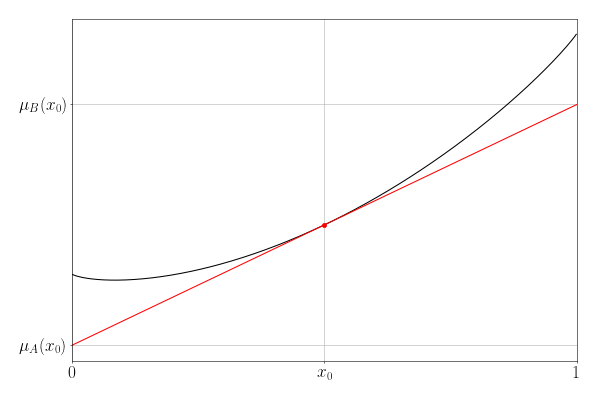
\includegraphics[width=\textwidth]{figures/Fig05a}
\end{minipage}\hfill\begin{minipage}{0.38\textwidth}
\captionof{figure}{Evolution de l'enthalpie libre molaire d'un mélange solide homogène avec la composition du mélange à température et pression fixé.}
\end{minipage}
\end{center}

\definition{Dans une phase donnée, le tracé de la tangente de la fonction enthalpie libre molaire en $x_0$ permet de lire le potentiel chimique du constituant \ce{A} (resp. \ce{B}) dans cette phase à la composition $x_0$.}

La conséquence mathématique pratique de cette définition est que la différence des potentiels chimiques $\mu_B - \mu_A$ correspond à la pente de la tangente à l'enthalpie libre molaire, tandis que le potentiel chimique de \ce{A} correspond à l'ordonnée à l'origine de cette tangente : 
\begin{align*}
\mu_B (T, P, x_0) - \mu_A (T, P, x_0) &= \left( \frac{\partial \bar{G}}{\partial x} \right)_{T, P, x_0} (T, P, x_0)\\
\mu_A (T, P, x_0) &= \bar{G} (T, P, x_0) - x_0 \left( \frac{\partial \bar{G}}{\partial x} \right)_{T, P, x_0} (T, P, x_0)
\end{align*}
De même avec le potentiel chimique de \ce{B} :
\begin{align*}\mu_B (T, P, x_0) &= \bar{G} (T, P, x_0) + (1-x_0) \left( \frac{\partial \bar{G}}{\partial x} \right)_{T, P, x_0} (T, P, x_0)
\end{align*}

\paragraph{Comparaison d'un système hétérogène et d'un système homogène}

Les courbes d'enthalpies libre nous permettent en général d'interpréter l'existence, ou non, de une ou plusieurs phases à un composition donnée. Lorsque la courbe d'une phase homogène est connue, on peut facilement comparer l'enthalpie libre d'un mélange homogène à celle d'un mélange mélange hétérogène.


\begin{center}
\begin{minipage}{0.58\textwidth}
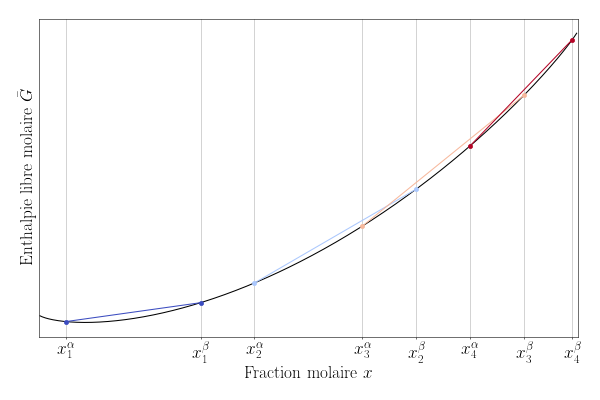
\includegraphics[width=\textwidth]{figures/Fig05b}
\end{minipage}\hfill\begin{minipage}{0.38\textwidth}
\captionof{figure}{Evolution de l'enthalpie libre de mélange dans un solide décrit par un modèle de solution régulière}
[$4$ cordes représentant $4$ mélanges hétérogènes, qui sont moins stables que le mélange homogène]
\label{fig:05b}
\end{minipage}
\end{center}

En particulier, lorsque l'on écrit l'équation d'une corde de l'enthalpie libre molaire : 
\begin{align*}
\bar{G}(T, P, x) &= \frac{\bar{G}(T, P, x_B^\beta) - \bar{G}(T, P, x_B^\alpha)}{x_B^\beta - x_B^\alpha} \cdot (x - x_B^\alpha) + \bar{G}(T, P, x_B^\alpha) \\
&= \bar{G} (T, P, x_B^\beta) x^\beta + \bar{G} (T, P, x_B^\alpha) \underbrace{(1 - x^\beta)}_{x^\alpha} \quad \text{car } x^\beta = \frac{x - x_B^\alpha}{x_B^\beta - x_B^\alpha} \text{ d'après le théorème des moments}
\end{align*}

On se rend compte que l'on retrouve l'expression de l'enthalpie libre d'un mélange hétérogène constitué d'une fraction $1 - x^\beta$ d'une phase $\alpha$ et d'une fraction $x^\beta$ d'une phase $\beta$.

\`{A} la Fig. \ref{fig:05b}, on observe que l'enthalpie libre molaire est une fonction convexe. Par conséquent, l'enthalpie libre d'un mélange hétérogène est toujours supérieure à celle du mélange homogène. La fonction représentée ne pourrait que représenter une phase homogène.

\definition{
Le tracé d'une corde sur le segment $[x_B^\alpha, x_B^\beta]$ d'une fonction enthalpie libre représente l'évolution de l'enthalpie libre d'un mélange hétérogène constitué d'une phase $\alpha$ composée d'une fraction $x_B^\alpha$ en constituant \ce{B} et d'une phase $\beta$ composée d'une fraction $x_B^\beta$ en constituant \ce{B}.
}

\subsection{Exemple de la démixtion}

Pour qu'une démixtion puisse exister, il faut que la fonction enthalpie libre présente des régions concaves.

En effet, dans la Fig. \ref{fig:05c}, le segment (1) et (3) présentent des cordes d'enthalpies libre supérieure au mélange homogène. Par conséquent, sur la région (1) (resp. (3)), le mélange forme une solution solide enrichie en \ce{A} (resp. en \ce{B}). Par contre, dans le segment (2), on remarque que la corde est sous la courbe d'énergie libre. Par conséquent, la réaction de démixtion est spontanée (favorable), c'est-à-dire que le mélange hétérogène est plus stable que le mélange homogène. 

\begin{center}
\begin{minipage}{0.58\textwidth}
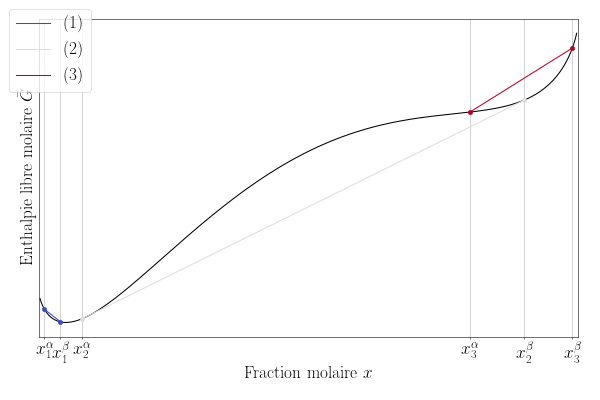
\includegraphics[width=\textwidth]{figures/Fig05c}
\end{minipage}\hfill\begin{minipage}{0.38\textwidth}
\captionof{figure}{Allure de l'enthalpie libre conduisant à un système solide-solide partiellement miscible.}
[Corde {\color{blue}(1)} et {\color{red}(3)} représentant des mélanges hétérogènes moins stables que le mélange homogène, corde {\color{gray}(2)} représentant un mélange hétérogène plus stable que le mélange homogène]
\label{fig:05c}
\end{minipage}
\end{center}

Un système évoluant vers le mélange hétérogène le plus stable se traduit graphiquement par la corde de plus basse enthalpie. Lorsque l'on minimise l'enthalpie de la corde, on trouve que la solution mathématique est une tangente commune au point de composition $x_B^\alpha$ et $x_B^\beta$ (assez intuitif du point de vu géométrique).

En effet, à l'équilibre chimique, les potentiels chimiques de \ce{A} et \ce{B} dans la phase $\alpha$ doivent être égaux à ceux de la phase $\beta$ :
\begin{align*}
  \begin{cases} \ce{A (\alpha) <=> A(\beta)} \\
  \ce{B (\alpha) <=> B(\beta)}
  \end{cases}  
  \iff 
  \begin{cases}
  \mu_A^\alpha (T, P, x_B^\alpha) &= \mu_A^\beta (T, P, x_B^\beta) \\
  \mu_B^\alpha (T, P, x_B^\alpha) &= \mu_B^\beta (T, P, x_B^\beta)
  \end{cases} \\
  \iff \mu_B^\alpha (T, P, x_B^\alpha) - \mu_A^\alpha (T, P, x_B^\alpha) = \mu_B^\beta (T, P, x_B^\beta) - \mu_A^\beta (T, P, x_B^\beta) \\
  \iff \left( \frac{\partial \bar{G}}{\partial x} \right)_{T, P, x_B^\alpha} (T, P, x_B^\alpha)= \left( \frac{\partial \bar{G}}{\partial x} \right)_{T, P, x_B^\beta} (T, P, x_B^\beta)
\end{align*}

Comme $\bar{G} (T, P, x) = (1-x) \mu_A (T, P, x) + x \mu_B (T, P, x)$, on trouve que :
\begin{align*}\left( \frac{\partial \bar{G}}{\partial x} \right)_{T, P, x_B^\alpha} (T, P, x_B^\alpha) &= \left( \frac{\partial \bar{G}}{\partial x} \right)_{T, P, x_B^\beta} (T, P, x_B^\beta) \\
&= \frac{\bar{G} (T, P, x_B^\beta) - \bar{G} (T, P, x_B^\alpha)}{x_B^\beta - x_B^\alpha}
\end{align*}

\definition{
Lorsqu'il y a coexistence de deux phases, la composition $x_B^\alpha$ et $x_B^\beta$ conduisant au mélange (à la corde) le plus stable correspond à une tangente commune au point $x_B^\alpha$ et $x_B^\beta$.
}

\section{Diagramme binaire à fuseau idéal}

Dans cette section, on va voir comment faire la relation entre l'enthalpie libre et les courbes de liquidus et solidus d'un diagramme binaire à fuseau idéal.

\subsection{Equations du liquidus et solidus}

\subsubsection{Transformation étudiée}
\definition{
On va considèrer le refroidisement d'un liquide homogène et idéal à toute composition qui conduit à un phenomène de solidification en un solide homogène : 
\begin{align*}
\ce{A(l) &-> A(s)} \\
\ce{A(l) &-> B(s)}
\end{align*}
La phase solide $(s)$ est une solution solide $\ce{A_{1-x} B_x}$. 
}

Lors de l'étude, on sera emmené à poser des approximations concernant les enthalpies de fusion : 
\begin{align*}
\Delta_{fus} H^\circ (T) &= \Delta_{fus} H^\circ (T_{fus}^\star) + \int_{T_{fus}^\star}^T C_{P,l} (T') - C_{P, s} (T') dT' \\
&\approx \Delta_{fus} H^\circ (T_{fus}^\star) + (C^\circ_{P,l} - C_{P, s}^\circ )(T - T_{fus}^\star) \\
&\approx \Delta_{fus} H^\circ (T_{fus}^\star)
\end{align*}

Dans le cas où les solides étudiés ont une capacité thermique indépendante de la température, et que leurs capacités thermiques sont similaires, on peut considérer que la température de fusion est relativement indépendante de la température.

Ceci est raisonnablement vérifié : 
\begin{itemize}
\item à des températures proches de la température de fusion, on est bien au-dessus de la température de Debye par conséquent la capacité peut-être considérée comme constante (pour les métaux);
\item pour des solutions solides, puisque les températures de fusion sont nécessairement relativement proches, ce qui traduit une faible plage de température pour la transformation comprises entre les deux températures de fusion des corps purs \ce{A} et \ce{B}.
\end{itemize}

De plus, nous supposerons que le liquide et le solide sont incompressibles, ce qui implique que le volume molaire du solide ne dépend pas de la pression. Par conséquent, le potentiel chimique des constituants peuvent se réduire à : 
\begin{align*}
\mu_s^\star (T, P) \approx \mu_s^{\star, \circ} (T)
\end{align*}

\subsubsection{Equation de Schröder-van Laar}

Lors de la transformation du mélange, on peut relater l'existence de 4 relations thermodynamique : 
\begin{enumerate}
\item équations de conservation de la matière : 
\begin{align*}
x_A^l + x_B^l &= 1 \\
x_A^s + x_B^s &= 1
\end{align*}
\item équilibres thermodynamique :
\begin{align*}
\mu_A^l (T, x_A^l) &= \mu_A^s (T, x_A^s) \\
\mu_B^l (T, x_B^l) &= \mu_B^s (T, x_B^s)
\end{align*}
\end{enumerate}

\definition{
En considérant une solution solide, incompressible et idéale, on aboutit aux équations de van Laar qui décrivent la composition de la phase solide et liquide : 
\begin{center}
\begin{tabular}{ccc}
\toprule
Constituant & Liquidus & Solidus \\
\midrule
A & $x_A^l (T) = \frac{e^{\lambda_B (T)} - 1}{e^{\lambda_B (T)} - e^{\lambda_A (T)}}$ & $x_A^s (T) = e^{\lambda_A (T)} \frac{1 - e^{\lambda_B (T)}}{e^{\lambda_A (T)} - e^{\lambda_B (T)}}$ \\
B & $x_B^l (T) = \frac{e^{\lambda_A (T)} - 1}{e^{\lambda_A (T)} - e^{\lambda_B (T)}}$ & $x_B^s (T) = e^{\lambda_B (T)} \frac{1 - e^{\lambda_A (T)}}{e^{\lambda_B (T)} - e^{\lambda_A (T)}}$\\
\bottomrule
\end{tabular}
\end{center}

En notant :
\begin{align*}
\lambda_A (T) &= \frac{\Delta_{fus} H^\circ ( T^\star_{fus,A})}{R} \left( \frac{1}{T} - \frac{1}{T^\star_{fus,A}} \right) \\
\lambda_B (T) &= \frac{\Delta_{fus} H^\circ ( T^\star_{fus,B})}{R} \left( \frac{1}{T} - \frac{1}{T^\star_{fus,B}} \right)
\end{align*}}

\attention{
Pour démontrer, vous aurez besoin d'établir une relation entre l'enthalpie libre et l'enthalpie, appelée relation de Gibbs-Helmholtz :
\begin{align*}
  \left( \frac{\partial (G/T)}{\partial T} \right)_{P} = - \frac{H}{T^2}
\end{align*}
en vous appuyant sur les identités thermodynamiques.
}

\subsection{Comparaison à quelques données expérimentales}

Les systèmes présentant un unique fuseau, peu déformé, comme à la Fig. \ref{fig:02a} est relativement bien décrit, en général, par une solution idéale.

\begin{center}
\begin{minipage}{0.58\textwidth}

\includegraphics[width=\textwidth]{figures/Fig02a}
\end{minipage}\hfill\begin{minipage}{0.38\textwidth}
\captionof{figure}{Diagramme isobare \ce{Cu}-\ce{Ni} à une pression de \SI{1}{\bar} modélisée à l'aide de l'équation de Schröder-van Laar}\label{fig:02a}
\begin{center}
\begin{tabular}{ccc}
\toprule
Element & Temp. fusion & Enthalpie de fusion \\
& \si{\kelvin} & \si{\kilo\joule\per\mole} \\
\midrule
\ce{Ni} & 1353.4 & 13.26 \\
\ce{Cu} & 1728 & 17.48 \\
\bottomrule
\end{tabular}
\captionof{table}{Paramètres du modèle}
\end{center}
\end{minipage}
\end{center}

L'écart observé ici résulte du fait que l'enthalpie de fusion est supposée indépendante de la température. Ce qui ici est plutôt une hypothèse abérrante au vu de la différence de température de fusion entre le nickel et le cuivre.

D'autres systèmes sont éloignés de l'idéalité, comme le système \ce{Au-Pt}, qui bien qu'ayant la même structure et des rayon atomiques proches, présentent un comportement non idéal.

\begin{center}
\begin{minipage}{0.58\textwidth}

\includegraphics[width=\textwidth]{figures/Fig02b}
\end{minipage}\hfill\begin{minipage}{0.38\textwidth}
\captionof{figure}{Diagramme isobare \ce{Au}-\ce{Pt} à une pression de \SI{1}{\bar} modélisée à l'aide de l'équation de Schröder-van Laar}\label{fig:02b}
\begin{center}
\begin{tabular}{ccc}
\toprule
Element & Temp. fusion & Enthalpie de fusion \\
& \si{\kelvin} & \si{\kilo\joule\per\mole} \\
\midrule
\ce{Au} & 1337.6 & 12.7 \\
\ce{Pt} & 2045.2 & 21.8 \\
\bottomrule
\end{tabular}
\captionof{table}{Paramètres du modèle}
\end{center}
\end{minipage}
\end{center}

Comme le montre la Fig. \ref{fig:02b}, le système se comporte de manière quasi-idéal pour des fractions en platine $x_{\ce{Pt}} < 0.10$ et $x_{\ce{Pt}} > 0.95$. En dehors de ces deux domaines, le système présente des interactions \ce{Pt-Au} beaucoup moins stables que les interactions \ce{Pt-Pt} et \ce{Au-Au}.

\definition{La comparaison d'une situation d'idéalité avec les données expérimentales permet d'interpréter l'écart d'intensité des interactions \ce{A-A}/\ce{B-B} et \ce{A-B}.

L'existence de deux fuseaux avec un point indifférent plus bas que les températures de fusion des corps purs signifie que les interactions \ce{A-B} sont beaucoup moins stable que les interactions \ce{A-A} et \ce{B-B}.

Dans le cas où le point indifférent est plus haut que les températures de fusion, l'interprétation est inverse. 
}

Bien entendu, il est possible d'affiner le modèle de solution régulière qui donne des résultats appréciables dans plusieurs alliages. 

\subsection{Influence de paramètres expérimentaux sur la forme des fuseaux}

Comme représenté à la Fig. \ref{fig:02d}, dans un mélange homogène, plus l'enthalpie de fusion du corps pur le plus stable est grande, plus la fusion débute et termine à des températures élevées.

\begin{center}
\begin{minipage}{0.58\textwidth}
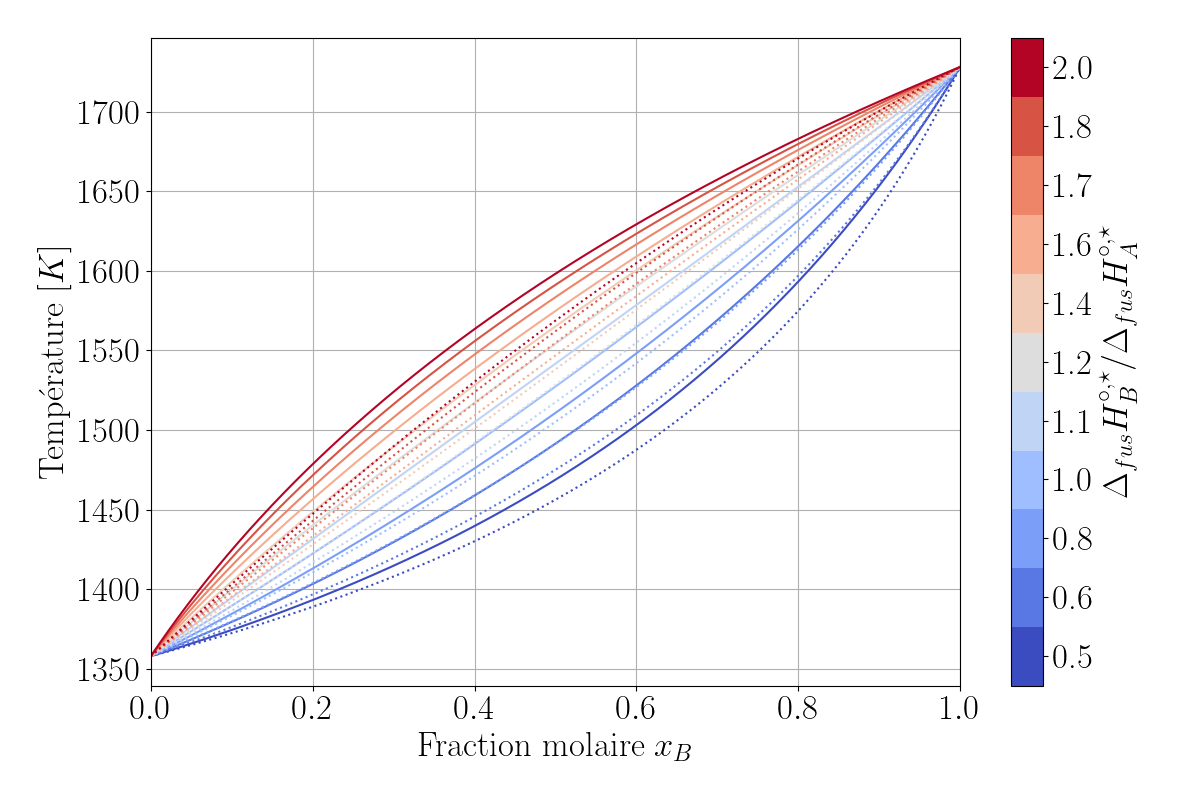
\includegraphics[width=\textwidth]{figures/Fig02d}
\end{minipage}\hfill\begin{minipage}{0.38\textwidth}
\captionof{figure}{Influence du rapport des enthalpies de fusion sur la forme du fuseau idéal}
\label{fig:02d}
\end{minipage}
\end{center}

Comme représenté à la Fig. \ref{fig:02e}, dans un mélange homogène, la différence de stabilité entre les deux corps pur a une influence sur la plage de température de fusion. En effet, plus les températures de fusion des corps purs sont proches, plus il y a de chance que la fusion ait lieu à une plage étroite de température. 

\begin{center}
\begin{minipage}{0.58\textwidth}
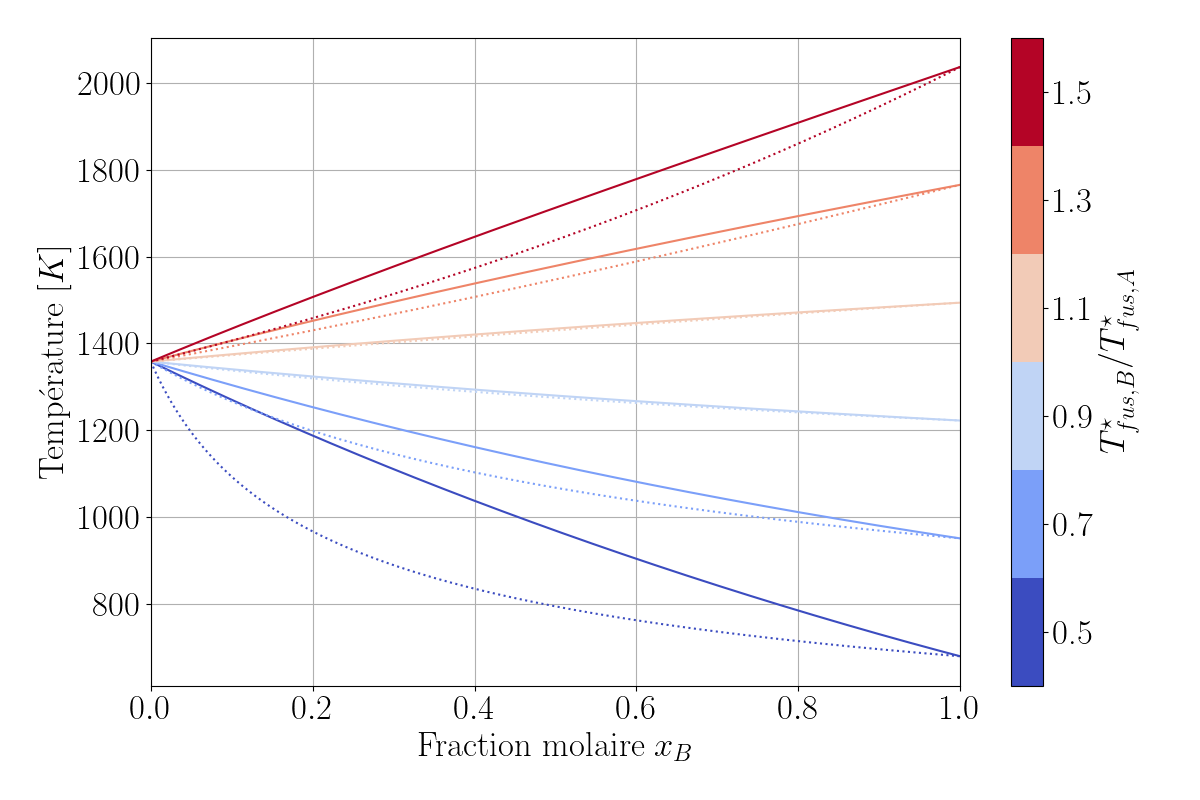
\includegraphics[width=\textwidth]{figures/Fig02e}
\end{minipage}\hfill\begin{minipage}{0.38\textwidth}
\captionof{figure}{Influence du rapport des températures de fusion sur la forme du fuseau idéal}
\label{fig:02e}
[les enthalpies de fusion sont celles du couple \ce{Ni}-\ce{Cu}]
\end{minipage}
\end{center}

Une conséquence immédiate est qu'il est extrêmement difficile de séparer deux composants de températures de fusion proche par cristallisation fractionnée.

\section{Diagramme binaire hétérogène idéal à miscibilité nulle}

On considère un mélange hétérogène, entre deux phases parfaitement non miscibles \ce{A(s)} et \ce{B(s)}, décrites par les variables d'état $P, ~ T, ~ x_A^l, ~ x_A^s, ~ x_B^l$ et $x_B^s$.

Dans ce système, on peut relater 5 relations thermoynamique :
\begin{enumerate}
\item équations de conservation de la matière :
\begin{align*}
x_A^l + x_B^l &= 1 \\
x_A^s &= 1 \\
x_B^s &= 1
\end{align*}
\item équilibres thermodynamiques :
\begin{align*}
\mu_A^l (T, x_A^l) &=  \mu_A^s (T, x_A^s) \\
\mu_B^l (T, x_B^l) &=  \mu_B^s (T, x_B^s)
\end{align*}
\end{enumerate}
 
Les équations du solidus sont assez directes à établir dans un mélange hétérogène à miscibilité nulle : 
\begin{align*}
\forall T > T_E, \begin{cases}
x_A^s (T) &= 1 \\
x_B^s (T) &= 1 
\end{cases}
\end{align*}

\subsection{Equations du liquidus}

La démarche à suivre est relativement similaire à celle utilisée pour établir les équations du liquidus dans un mélange homogène idéal.

\definition{
dans un système hétérogène idéal, l'équation du liquidus s'écrit sous la forme : 
\begin{align*}
x_b^l (t) = \begin{cases}
1 - \exp \left( \frac{\delta_{fus} h_a^\circ}{r} \left( \frac{1}{t_{fus,a}^\star} - \frac{1}{t}\right) \right) \text{ si } x_b (t) < x_e \\
\exp \left( \frac{\delta_{fus} h_b^\circ}{r} \left( \frac{1}{t_{fus,b}^\star} - \frac{1}{t}\right) \right) \text{ si } x_b (t) > x_e
\end{cases}
\end{align*}

La température eutectique se détermine à l'intersection des deux liquidus : 
\begin{align*}
1 - \exp \left( \frac{\Delta_{fus} H_A^\circ}{R} \left( \frac{1}{T_{fus,A}^\star} - \frac{1}{T_E}\right) \right) = \exp \left( \frac{\Delta_{fus} H_B^\circ}{R} \left( \frac{1}{T_{fus,B}^\star} - \frac{1}{T_E}\right) \right)
\end{align*}
}



\subsection{Comparaison à quelques données expérimentales}

Prenons le système \ce{AgCl-ZnCl2}, où les deux corps purs présentent des structures cristallographiques et des cations de valences distinctes. 

\begin{center}
\begin{minipage}{0.58\textwidth}

\includegraphics[width=\textwidth]{figures/Fig03a}
\end{minipage}\hfill\begin{minipage}{0.38\textwidth}
\captionof{figure}{Diagramme de phase d'un solide hétérogène \ce{AgCl}-\ce{ZnCl2} à miscibilité nulle, isobare, à une pression de \SI{1}{\bar}}\label{fig:03a}
\begin{center}
\begin{tabular}{ccc}
\toprule
Element & Temp. fusion & Enthalpie de fusion \\
& \si{\kelvin} & \si{\kilo\joule\per\mole} \\
\midrule
\ce{ZnCl2} & 587 & 22.95 \\
\ce{AgCl} & 728 & 8.500 \\
\bottomrule
\end{tabular}
\captionof{table}{Paramètres du modèle}
\end{center}
\end{minipage}
\end{center}

En considérant que le système se comporte de manière idéal et en utilisant les paramètres de fusion des corps purs, on retrouve un accord relativement correct entre les courbes de liquidus modélisées et expérimentales.

La température eutectique, obtenue à l'intersection des deux courbes liquidus vaut $T_E = 504 ~ \si{\kelvin}$. Le point eutectique correspond à une composition eutectique en \ce{B} $x_E = 0.54$. Ces grandeurs sont en bon accord avec les données expérimentales.

\subsection{Influence de paramètres expérimentaux sur la forme des fuseaux}

La Fig. \ref{fig:03b} montre que le domaine liquide + \ce{B(s)} est d'autant plus grand que la température de fusion de \ce{B} est grand. 

\begin{center}
\begin{minipage}{0.58\textwidth}

\includegraphics[width=\textwidth]{figures/Fig03b}
\end{minipage}\hfill\begin{minipage}{0.38\textwidth}
\captionof{figure}{Influence du rapport des enthalpies de fusion sur la forme du diagramme binaire non miscible}
[l'enthalpie de fusion de \ce{A(s)} est constante]
\label{fig:03b}
\end{minipage}
\end{center}

Par conséquent, la température eutectique est d'autant plus haute que les composés purs ont une enthalpie de fusion élevée. Si le composé \ce{B} (resp. \ce{A}) a une grande enthalpie de fusion, la composition eutectique diminue (resp. augmente).

\begin{center}
\begin{minipage}{0.58\textwidth}
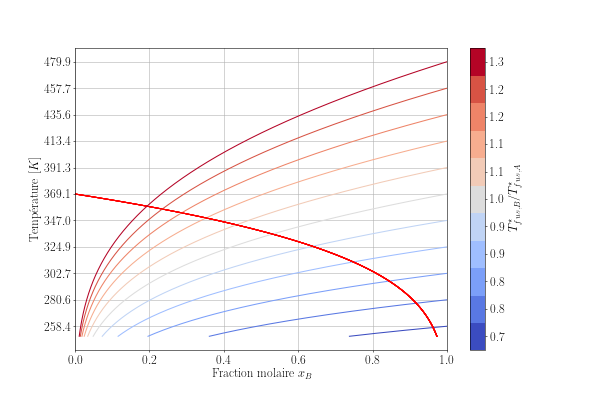
\includegraphics[width=\textwidth]{figures/Fig03c}
\end{minipage}\hfill\begin{minipage}{0.38\textwidth}
\captionof{figure}{Influence du rapport des températures de fusion sur la forme du diagramme binaire non miscible}
[la température de fusion de \ce{A(s)} est constante]
\label{fig:03c}
\end{minipage}
\end{center}

Comme le montre la Fig. \ref{fig:03c}, le rapport de la température de fusion des corps purs suit exactement les mêmes tendances que le rapport d'enthalpies de fusion.



\end{document}
